% !TeX root = ../jvk-blatt0.tex

\excercise{JDK installieren}
\label{ex1}
Um Java benutzen zu können musst du nun noch eine JDK herunterladen. Dies kannst du ganz einfach direkt in IntelliJ tun indem du Strg+Alt+Shift+S drückst und den auf dem Bild 1 ausgewählten Reiter auswählst.
\begin{center}
    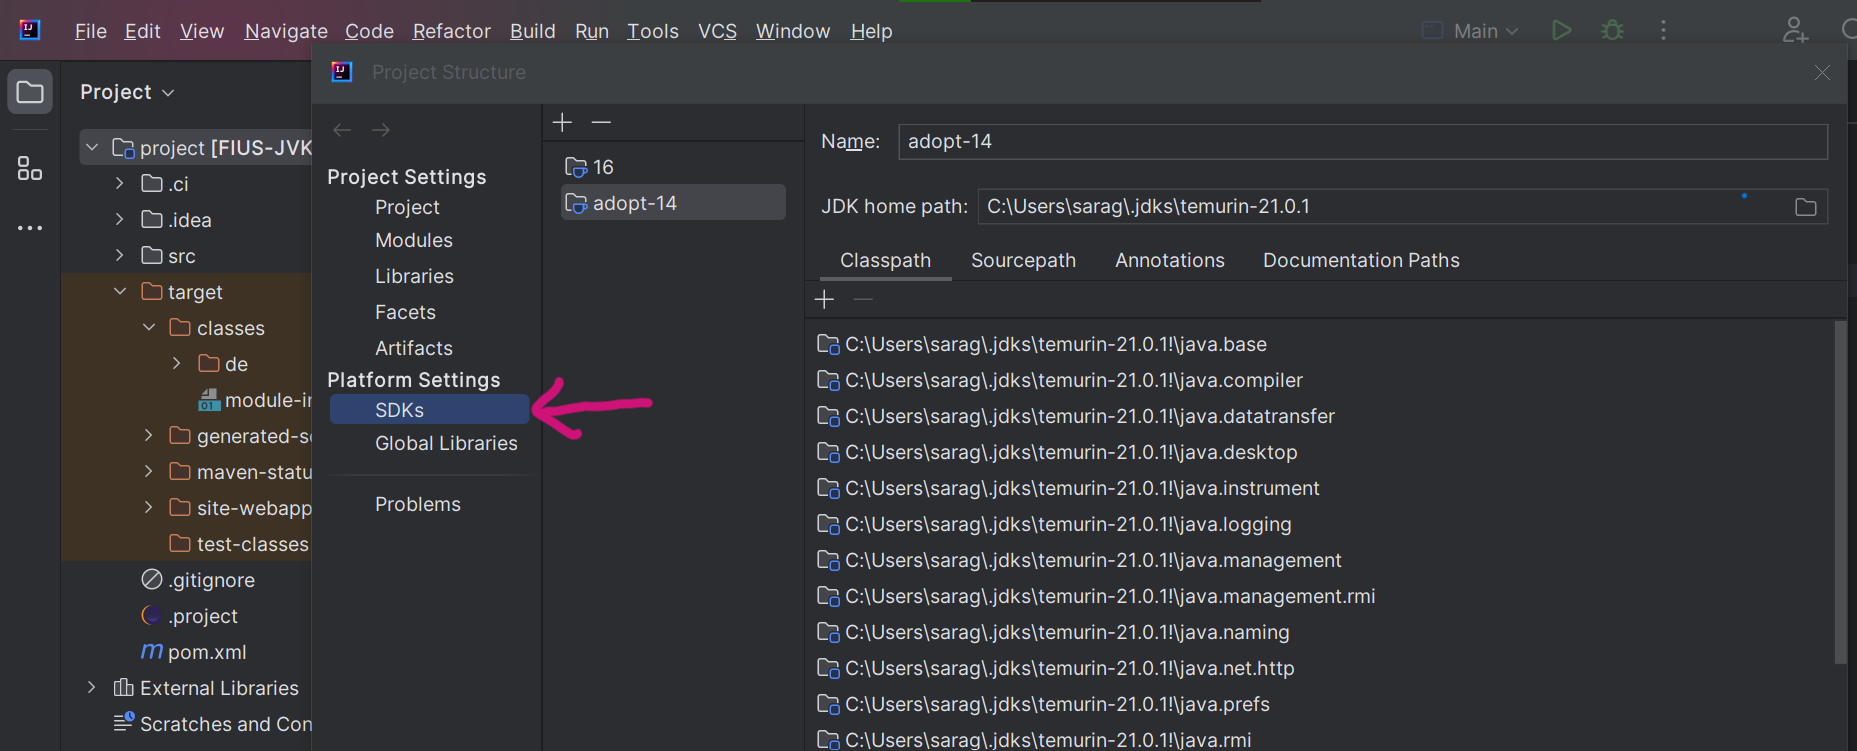
\includegraphics[width=\linewidth]{./3/IntelliJ JDK.PNG}
\end{center}
Nun musst du entweder eine schon installierte JDK auswählen oder neue installieren. Um eine neue JDK zu installieren musst die beiden auf Bild 2 markierten Dinge anklicken. Nun wird sich ein Fenster wie das in Bild 3 öffnen.
\begin{center}
    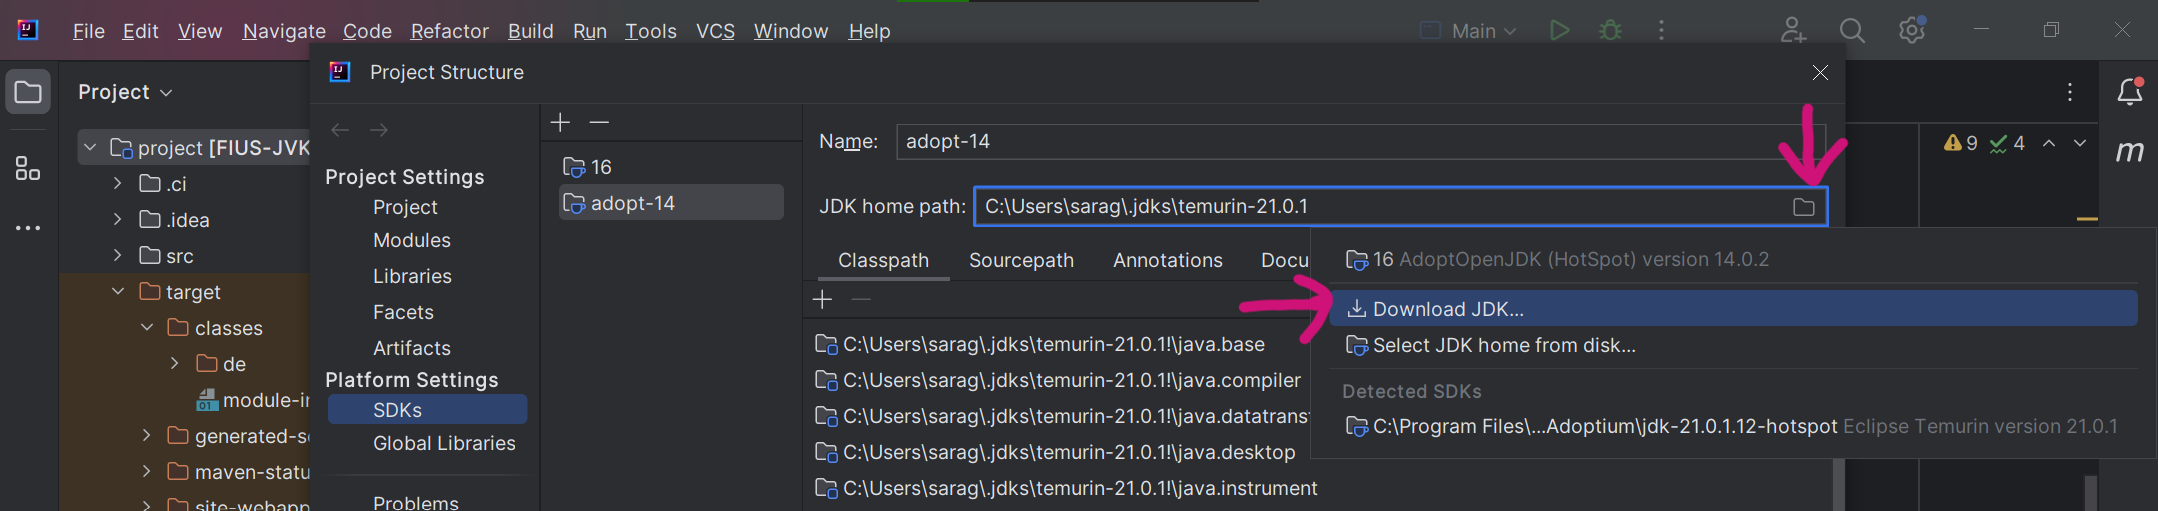
\includegraphics[width=\linewidth]{./3/IntelliJ JDK 2.PNG}
\end{center}
\newpage
Installiere nun die auf dem Bild 3 gezeigte Version und füge einen sinnvollen Speicherort hinzu.
\begin{center}
    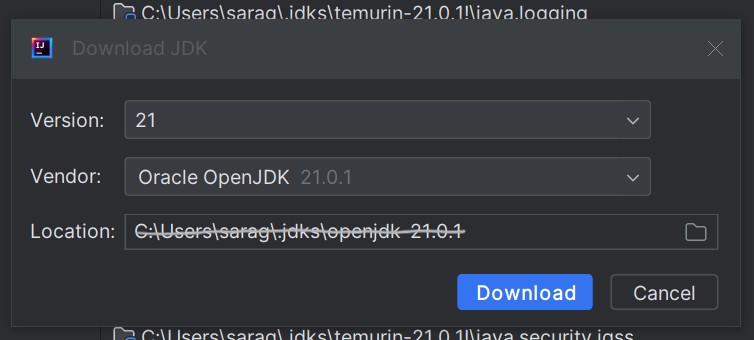
\includegraphics[width=\linewidth]{./3/IntelliJ JDK 3.PNG}
\end{center}
